%% zusammenf.tex
%% $Id: zusammenf.tex 61 2012-05-03 13:58:03Z bless $
%%

\chapter{Zusammenfassung und Ausblick}
\label{ch:Zusammenfassung}
%% ==============================
Zusammenfassend l"asst sich also sagen, dass es heute viele M"oglichkeiten gibt, Daten zu speichern. Die einen sind praktischer, die anderen etwas unpraktischer.
Der meist genutzte Massenspeicher ist im Moment wohl die Festplatte, seine Entwicklung war rasant – "ahnlich dem \textit{Mooreschen Gesetz} zeigt sie einen ann"ahernd exponentiellen Verlauf wie die Abbildung \ref{fig:kapazit} zeigt. Alle 16 Monate etwa, verdoppelt sich damit die Speicherkapazit"at
\begin{figure}[ht]
				\centering
				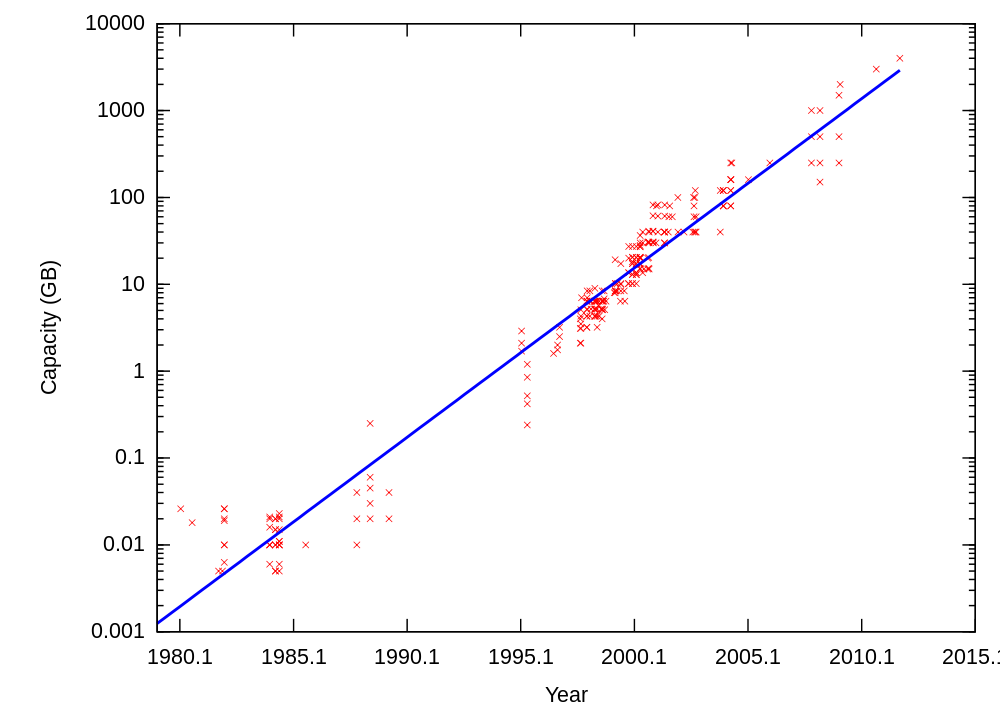
\includegraphics[width=0.7\textwidth]{images/kapazit} 
				\caption[Entwicklung Speicherkapazit"at Fesplatte in halblogarithmischer Skalierung \cite{fig:kapazit}]{Entwicklung Speicherkapazit"at Fesplatte in halblogarithmischer Skalierung}
				\label{fig:kapazit}
				\end{figure}
\\
Auch die Rohstoffverknappung k"onnte den Speicherhunger behindern, wie die Flutkatastrophe Ende 2011 in Thailand zeigte. Die Preise f"ur Festplatten stiegen darauf hin, da nahezu alle Festplatten der Marktriesen dort produziert wurden.
\\
Doch irgendwann wird die physikalische Grenze erreicht werden.
\\
Das Ziel ist es 1 Bit mit einem 1 Atom zu repr"asentieren, das Speichern auf atomarer Ebene. Im Januar 2012 konnten die Forscher des IBM Almaden Research Centers zusammen mit Forschern der Max-Planck-Gesellschaft den kleinsten Speicher der Welt bauen. Sie haben es geschafft einen 12 Atom Speicher zu bauen, allerdings ist dieser nur bei -268 Grad zuverl"assig. Bis er bei Raumtemperaturen funktioniert und Marktreif ist, wird es wohl noch einige Zeit dauern.\cite{heise:ibm} 
\\
Dann wird es aber wohl m"oglich sein die gesamte Weltliteratur auf einen Speicher von der Gr"o"se einer Briefmarke zu speichern. 

%%% Local Variables: 
%%% mode: latex
%%% TeX-master: "thesis"
%%% End: 
